\documentclass[12pt,a4paper]{report}

\usepackage{alltt, fancyvrb, url}
\usepackage{graphicx}
\usepackage[utf8]{inputenc}
\usepackage{float}
\usepackage{xcolor}
\usepackage{hyperref}
\usepackage{longtable}
\usepackage{listings}

\definecolor{codegreen}{rgb}{0,0.6,0}
\definecolor{codegray}{rgb}{0.5,0.5,0.5}
\definecolor{codepurple}{rgb}{0.58,0,0.82}
\definecolor{backcolour}{rgb}{0.95,0.95,0.92}

\lstdefinestyle{mystyle}{
    backgroundcolor=\color{backcolour},   
    commentstyle=\color{codegreen},
    keywordstyle=\color{magenta},
    numberstyle=\tiny\color{codegray},
    stringstyle=\color{codepurple},
    basicstyle=\ttfamily\footnotesize,
    breakatwhitespace=false,         
    breaklines=true,                 
    captionpos=b,                    
    keepspaces=true,                 
    numbers=left,                    
    numbersep=5pt,                  
    showspaces=false,                
    showstringspaces=false,
    showtabs=false,                  
    tabsize=2
}
\lstset{style=mystyle}

\usepackage{enumitem}
\usepackage{amsmath}
\usepackage{geometry}
\geometry{margin=1in}

\usepackage{newlfont}
\usepackage{gensymb}

\usepackage[italian]{babel}
\usepackage[italian]{cleveref}

\graphicspath{ {./src/img} }

\textwidth=450pt\oddsidemargin=0pt
\begin{document}

\begin{titlepage}
\begin{center}
{{\Large{\textsc{Alma Mater Studiorum $\cdot$ Università di Bologna}}}} \rule[0.1cm]{15.8cm}{0.1mm}
\rule[0.5cm]{15.8cm}{0.6mm}
{\small{\bf CORSO DI LAUREA IN INGEGNERIA E SCIENZE INFORMATICHE \\ A.A. 2024/25 }}
\end{center}
\vspace{15mm}
\begin{center}
{\LARGE{\bf Analisi del traffico ICMP e TCP}}\\
\vspace{2mm}
{\LARGE{\bf con Scapy e Wireshark}}
\end{center}
\begin{center}
{\LARGE Relazione per il corso di Programmazione di Reti}
\end{center}

\vspace{8mm}
\begin{center}
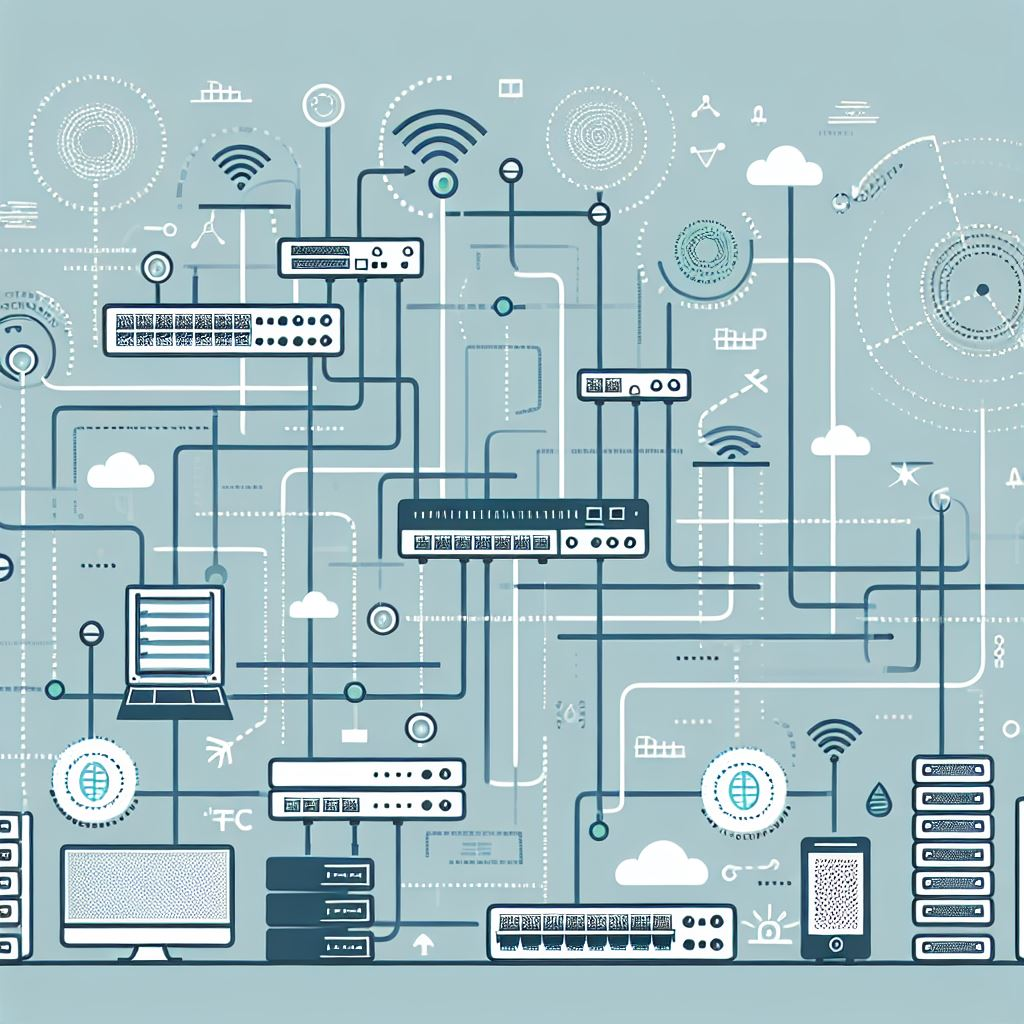
\includegraphics[width=0.7\textwidth]{Copertina}
\end{center}
\vspace{15mm}

{\large{\bf \noindent
Presentato da:\\}
Bartocetti Enrico, 0001115097}
\end{titlepage}

\tableofcontents

\chapter{Introduzione}

\subsubsection{Obiettivo}
Creare e inviare pacchetti ICMP e TCP con Scapy, catturarli con Wireshark e analizzare i risultati.

\subsubsection{Requisiti minimi}
\begin{itemize}
	\item Inviare pacchetti ICMP Echo (ping) e TCP SYN verso un host
	\item Catturare i pacchetti in Wireshark e salvarli in .pcap
	\item Analizzare: IP di origine/destinazione, porte, checksum, TTL
\end{itemize}

\subsubsection{Estensioni opzionali}
\begin{itemize}
	\item Inviare un pacchetto TCP con flag personalizzati
	\item Visualizzare e spiegare le differenze tra ICMP e TCP
	\item Generare un semplice report HTML o PDF con gli screen e analisi
\end{itemize}

\subsubsection{Output atteso}

\begin{itemize}
	\item Script Python con Scapy
	\item File .pcap della cattura
	\item Relazione con screenshot e commenti tecnici
\end{itemize}


\end{document}